\documentclass[a4paper, 12pt]{article}

\usepackage{graphicx}
\usepackage{longtable}
\graphicspath{ {images/} }

\newcommand{\templates}{../../template}
\usepackage[a4paper, margin=2.5cm]{geometry}

\usepackage{enumitem}
\setlist[itemize]{noitemsep}
\setlist[enumerate]{noitemsep}

\let\oldpar\paragraph
\renewcommand{\paragraph}[1]{\oldpar{#1\\}\noindent}
\usepackage{graphicx}
\usepackage{hyperref}
\usepackage{makecell}

\newcommand{\settitolo}[1]{\newcommand{\titolo}{#1\\}}
\newcommand{\setprogetto}[1]{\newcommand{\progetto}{#1\\}}
\newcommand{\setcommittenti}[1]{\newcommand{\committenti}{#1\\}}
\newcommand{\setredattori}[1]{\newcommand{\redattori}{#1\\}}
\newcommand{\setrevisori}[1]{\newcommand{\revisori}{#1\\}}
\newcommand{\setresponsabili}[1]{\newcommand{\responsabili}{#1\\}}
\newcommand{\setversione}[1]{
	\ifdefined\versione\renewcommand{\versione}{#1\\}
	\else\newcommand{\versione}{#1\\}\fi
}
\newcommand{\setdestuso}[1]{\newcommand{\uso}{#1\\}}
\newcommand{\setdescrizione}[1]{\newcommand{\descrizione}{#1\\}}

\newcommand{\makefrontpage}{
	\begin{titlepage}
		\begin{center}

		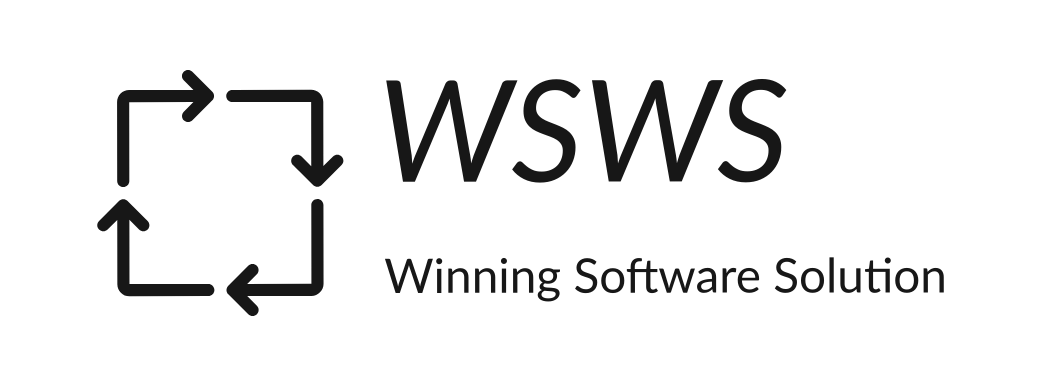
\includegraphics[width=0.4\textwidth]{../../template/WSWS-logos_transparent_crop}\\

		{\Large Winning Software Solution}\\[6pt]
		\href{mailto://winningsoftwaresolution@gmail.com}{winningsoftwaresolution@gmail.com}\\
		
		\ifdefined\progetto
		\vspace{1cm}
		{\Large\progetto}
		{\large\committenti}
		\else\fi
		
		\vspace{1.5cm}
		{\LARGE\titolo}
		
		\vfill
		
		\begin{tabular}{r | l}
		\multicolumn{2}{c}{\textit{Informazioni}}\\
		\hline
		
		\ifdefined\redattori
			\textit{Redattori} &
			\makecell[l]{\redattori}\\
		\else\fi
		\ifdefined\revisori
			\textit{Revisori} &
			\makecell[l]{\revisori}\\
		\else\fi
		\ifdefined\responsabili
			\textit{Respondabili} &
			\makecell[l]{\responsabili}\\
		\else\fi
		
		\ifdefined\versione
			\textit{Versione} & \versione
		\else\fi
		
		\textit{Uso} & \uso
		
		\end{tabular}
		
		\vspace{2cm}
		
		\ifdefined\descrizione
		Descrizione
		\vspace{6pt}
		\hrule
		\descrizione
		\else\fi
		\end{center}
	\end{titlepage}
}
\usepackage{hyperref}
\usepackage{array}
\usepackage{tabularx}

\def\vers#1-#2-#3-#4-#5\\{#1&#2&#3&#4&#5\\\hline}

\newcommand{\addversione}[5]{
	\ifdefined\versioni
		\let\old\versioni
		\renewcommand{\versioni}{#1&#2&#3&#4&#5\\\hline\old}
	\else
		\newcommand{\versioni}{#1&#2&#3&#4&#5\\\hline}
	\fi
}

\newcommand{\setversioni}[1]{\newcommand{\versioni}{#1}}

\newcommand{\makeversioni}{
	\begin{center}
		\begin{tabularx}{\textwidth}{|c|c|c|c|X|}
		\hline
		\textbf{Versione} & \textbf{Data} & \textbf{Persona} & \textbf{Attivtà} & \textbf{Descrizione} \\
		\hline
		\versioni
		\end{tabularx}
	\end{center}
	\clearpage
}

\settitolo{Analisi dei requisiti}
\setprogetto{ShopChain}
\setcommittenti{SyncLab}
\setredattori{Alberto Nicoletti, Andrea Volpe, Giovanni Cocco}
\setdestuso{esterno}
\setdescrizione{
Analisi dei requisiti del progetto ShopChain con casi d'uso e requisiti.
}

\addversione{0.0.0}{11/12/2021}{Alberto Nicoletti}{Redazione}{Struttura del documento, stesura sezioni 1 e 2}
\addversione{0.0.1}{30/12/2021}{Alberto Nicoletti}{Redazione}{Stesura casi d'uso da UC1 a UC5.4}
\addversione{0.0.2}{03/01/2022}{Andrea Volpe}{Redazione}{Stesura casi d'uso da UC6 a UC20}
\addversione{0.0.3}{03/01/2022}{Alberto Nicoletti}{Redazione}{Aggiunta immagini}
\addversione{0.0.4}{12/01/2022}{Andrea Volpe}{Redazione}{Modifica casi d'uso}
\addversione{0.0.5}{16/01/2022}{Alberto Nicoletti}{Redazione}{Stesura primi requisiti}
\addversione{0.0.6}{18/01/2022}{Andrea Volpe}{Redazione}{Stesura requisiti acquirente}
\addversione{0.0.7}{21/01/2022}{Alberto Nicoletti}{Redazione e correzione}{Riorganizzazione requisiti, aggiunta requisiti di vincolo e di qualità}
\addversione{0.0.8}{28/01/2022}{Andrea Volpe}{Correzione}{Correzione UC19 estensioni}
\addversione{0.0.9}{1/02/2022}{Alberto Nicoletti}{Correzione}{Correzzione immagini casi d'uso e requisiti}
\addversione{0.0.10}{03/02/2022}{Andrea Volpe}{Redazione e correzione}{Stesura RNO29 e correzione errori grammaticali}
\addversione{0.0.11}{04/02/2022}{Giovanni Cocco}{Correzione}{Correzioni varie}
\addversione{0.0.12}{05/02/2022}{Alberto Nicoletti}{Riscrittura}{Riscrittura di alcuni casi d'uso a seguito di una discussione interna al gruppo}

\begin{document}

\makefrontpage

\makeversioni

\section{Introduzone}
\subsection{Scopo del documento}
Lo scopo del documento è raccogliere i risultati dell'attività di analisi dei requisiti. Contiene quindi la descrizione dei casi d'uso del prodotto software da sviluppare, ed i requisiti suddivisi per tipologia. Si vuole così dimostrare una completa comprensione del problema e delle aspettative della soluzione. I casi d'uso, ma soprattuto i requisiti saranno tenunuti in considerazione nelle fasi di progettazione, di verifica e di validazione. 

\section{Descrizione del prodotto}
L'azieda \textit{SyncLab} propone, attraverso il capitolato C2: \textit{ShopChain - Exchange Platform on
BlockChain}. L'obiettivo è sviluppare un sistema che permetta ad un qualsiasi e-commerce di usare criptovalute come metodo di pagamento. Ciò consiste nella realizzazione su blockchain di una piattaforma che si incarichi di ricevere l’ammontare in criptovaluta, lo trattenga, e lo consegni al venditore solo quando il pacco viene recapitato all’acquirente.
\subsection{Scopo del prodotto}
Il progetto consiste nello sviluppo di una piattaforma su blockchain con lo scopo di rendere possibile l'acquisto di prodotti tramite criptovalute in sicurezza. Il processo di trasferimento del denaro avviene seguendo queste fasi:
\begin{enumerate}
\item caricamento dei dati dell'ordine di acquisto nella blockchain e generazione dello smart contract;
\item trasferimento del denaro dal wallet dell'acquirente in blockchain;
\item notifica al venditore dell'avvenuto pagamento e blocco del denaro in blockchain;
\item conferma di ricezione del pacco da parte dell'acquirente tramite scannerizzazione di un QR Code sul pacco del prodotto acquistato;
\item sblocco del denaro e trasferimento nel wallet del venditore.
\end{enumerate}
\subsection{Parti del prodotto}
Il prodotto software è composto dalle seguenti parti:
\begin{itemize}
\item smart contracts nella blockchain per la gestione di tutte le fasi del processo di trasferimento del denaro;
\item landing page per il pagamento da parte del acquirente;
\item piattaforma web per la visualizzazione e gestione delle transazioni sia da parte sia dell venditore che dell'acquirente;
\item webapp per la scannerizzazione del QR Code per la conferma ricezione pacco.
\end{itemize}
\subsection{Caratteristiche utenti}
Gli utenti di \textit{ShopChain} possono essere suddivisi in due categorie:
\begin{itemize}
\item venditore: gli amministratori di un sito di e-commerce che vogliono aggiungere le criptovalute come metodo di pagamento;
\item acquirente: I clienti di un sito di e-commerce che scelgono di utilizzare le criptovalute come pagamento per i prodotti da acquistare.
\end{itemize}
Tutti gli utenti sono in possesso di un wallet per criptovalute. 
Non potendo prevedere con accuratezza quanti e quali e-commerce decideranno di utilizzare \textit{ShopChain} altre considerazioni sulle caratteristiche di utenza sono superflue. Il prodotto deve essere facilmente integrabile in più tipologie di e-commerce possibili.

\subsection{Vincoli e preferenze}
Il proponente non impone vincoli nella scelta della tipologia di tecnologie, ma ci sono comunque delle scelte preferenziali da considerare:
\begin{itemize}
\item utilizzo di blockchain pubblica;
\item utilizzo di Java e Angular per lo sviluppo delle parti di Back-end e di Front-end della componente web application del sistema;
\item utilizzo di database PostgreSQL.
\end{itemize}

Per il completamento del progetto il proponente richiede che siano realizzati i seguenti risultati:
\begin{itemize}
\item server, completo di UI;
\item test che dimostrino il corretto funzionamento dei servizi e delle funzionalità previste, con una copertura minima dell'80\% correlata di report;
\item documentazione su scelte implementative e progettuali effettuate, le relative motivazioni, i problemi aperti e le eventuali soluzioni proposte da esplorare.
\end{itemize}

\section{Casi d'uso}

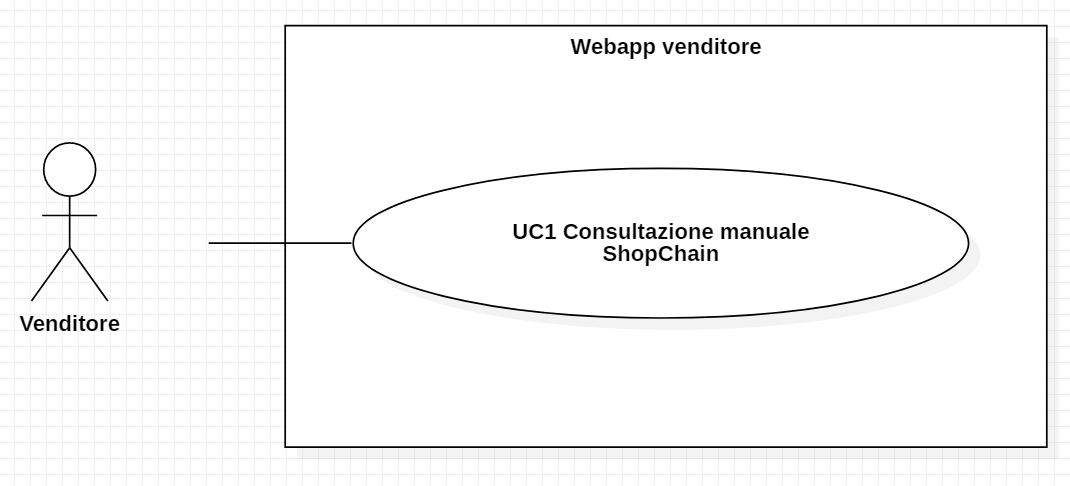
\includegraphics[width=0.7\textwidth]{UC_WAV1}

\paragraph{UC1 - Consultazione manuale ShopChain}\\
\textbf{Attori primari}: Venditore.\\
\textbf{Precondizioni}: Il venditore usa il servizio ShopChain e vorrebbe avere più informazioni sul suo utilizzo.\\
\textbf{Postcondizioni}: Il venditore consulta il manuale utente di ShopChain.\\
\textbf{Scenario principale}:\\
\begin{enumerate}
\item al venditore viene fornito il manuale utente già dall'acquisizione del prodotto ShopChain.
\item il venditore è libero di consultare il manuale in ogni momento.
\end{enumerate}

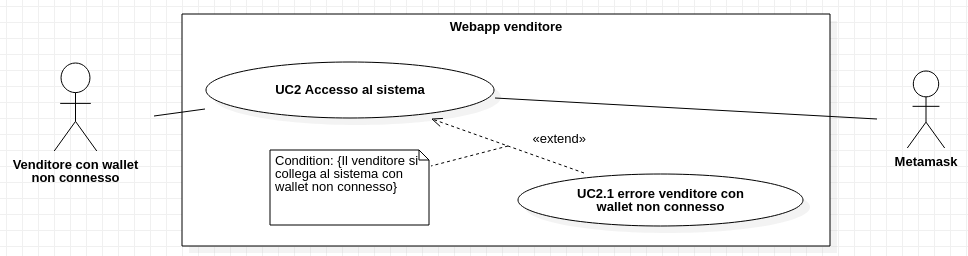
\includegraphics[width=0.9\textwidth]{UC_WAV2}

\paragraph{UC2 - Accesso al sistema (webapp venditore)}\\
\textbf{Attore primario}: Venditore con wallet non connesso.\\
\textbf{Attore secondario}: Metamask.\\
\textbf{Precondizioni}: Il venditore vuole accedere alla webapp.\\
\textbf{Postcondizioni}: Il venditore si è connesso alla web-app con metamask.\\
\textbf{Scenario principale}:
Il venditore usando Metamask, si connette alla webapp con il proprio wallet.

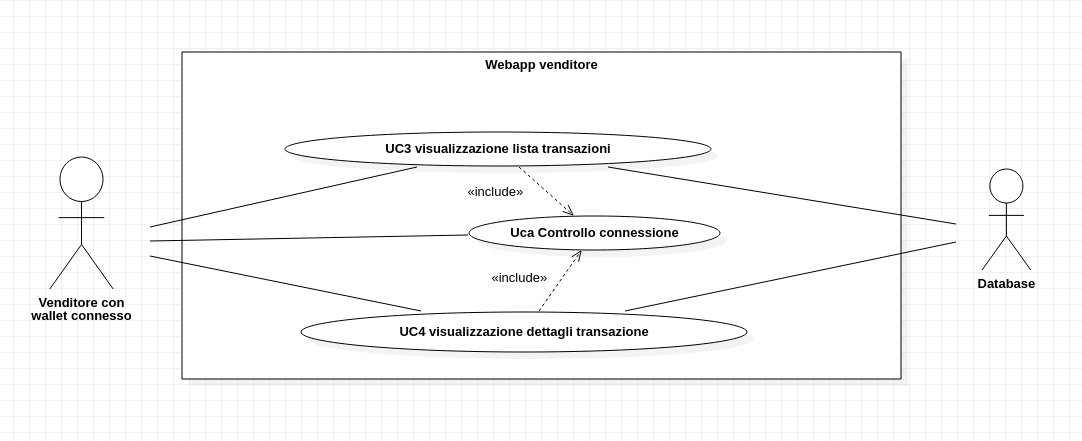
\includegraphics[width=0.9\textwidth]{UC_WAV3}

\paragraph{UC3 visualizzazione lista transazioni}\\
\textbf{Attore primario}: Venditore con wallet connesso. \\
\textbf{Attore secondario}: Database. \\
\textbf{Precondizioni}: Il venditore ha effettuato l'accesso al sistema.\\
\textbf{Postcondizioni}:  Il venditore vede la lista delle transazioni.\\
\textbf{Scenario principale}:
\begin{enumerate}
\item Il venditore vede la lista delle transazioni;
\item Il venditore può scegliere che tipo di transazioni vedere (tutte, completate, in attesa);
\item Il sistema mostra al venditore l'elenco delle transazioni richieste.
\end{enumerate}

\paragraph{UC4 - visualizzazione dettaglio transazione}\\
\textbf{Attore primario}: Venditore.\\
\textbf{Attore secondario}: Database.\\
\textbf{Precondizioni}: Il venditore ha acceduto alla funzionalità di visualizzazione della lista delle transazioni.\\
\textbf{Postcondizioni}: Il venditore vede i dettagli di una singola transazione.\\
\textbf{Scenario principale}:
\begin{enumerate}
\item il venditore seleziona una delle transazioni dall'elenco;
\item il venditore visualizza i dettagli della singola transazione.
\end{enumerate}

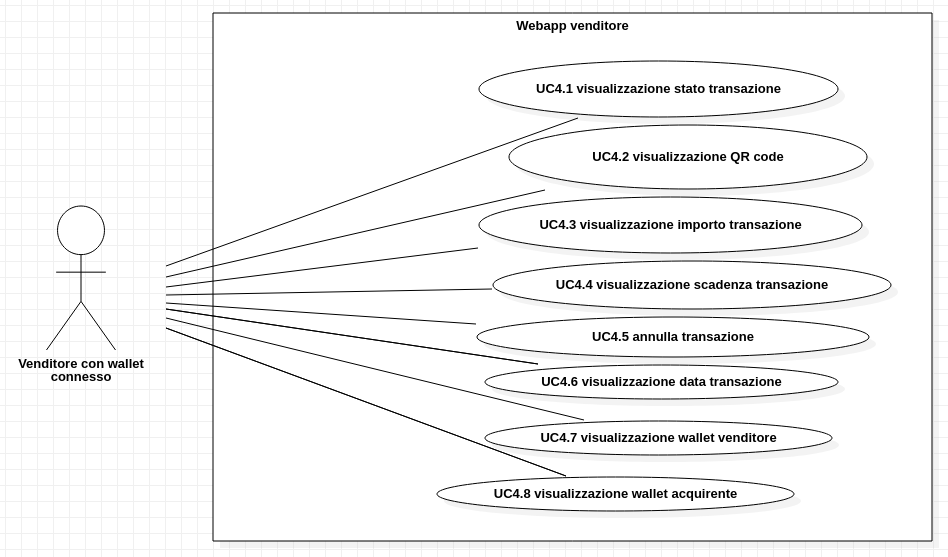
\includegraphics[width=0.9\textwidth]{UC_WAV4}

\paragraph{4.1 - Visualizzazione stato transazione}\\
\textbf{Attore primario}: Venditore con wallet connesso.\\
\textbf{Precondizioni}: Il venditore vuole visualizzare lo stato di una transazione.\\
\textbf{Postcondizioni}: Il venditore visualizza lo stato di una transazione.\\
\textbf{Scenario principale}: Il venditore vede se la transazione è in attesa, oppure è stata completata.\\

\paragraph{UC4.2 - Visualizzazione QR Code}\\
\textbf{Attore primario}: Venditore con wallet connesso.\\
\textbf{Precondizioni}: Il venditore vuole visualizzare il QR Code di una transazione in attesa.\\
\textbf{Postcondizioni}: Il venditore è in possesso del QR Code da applicare sul pacco del prodotto.\\
\textbf{Scenario principale}:
\begin{enumerate}
\item il venditore visualizza il QR Code della transazione in attesa selezionata;
\item il venditore stampa il QR Code lo applica sul pacco del prodotto.
\end{enumerate}

\paragraph{UC4.3 - Visualizzazione importo transazione}\\
\textbf{Attore primario}: Venditore con wallet connesso.\\
\textbf{Precondizioni}: Il venditore vuole visualizzare l'importo di una transazione.\\
\textbf{Postcondizioni}: Il venditore visualizza l'importo di una transazione.\\
\textbf{Scenario principale}: Il venditore vede l'importo della transazione.\\

\paragraph{UC4.4 - Visualizzazione scadenza transazione}\\
\textbf{Attore primario}: Venditore  con wallet connesso.\\
\textbf{Precondizioni}: Il venditore vuole visualizzare la scadenza di una transazione in attesa.\\
\textbf{Postcondizioni}: Il venditore visualizza la scadenza di una transazione in attesa.\\
\textbf{Scenario principale}: Il venditore vede la data della scadenza di una transazione in attesa, oltre la quale l'acquirente riceverà indietro la valuta bloccata.\\

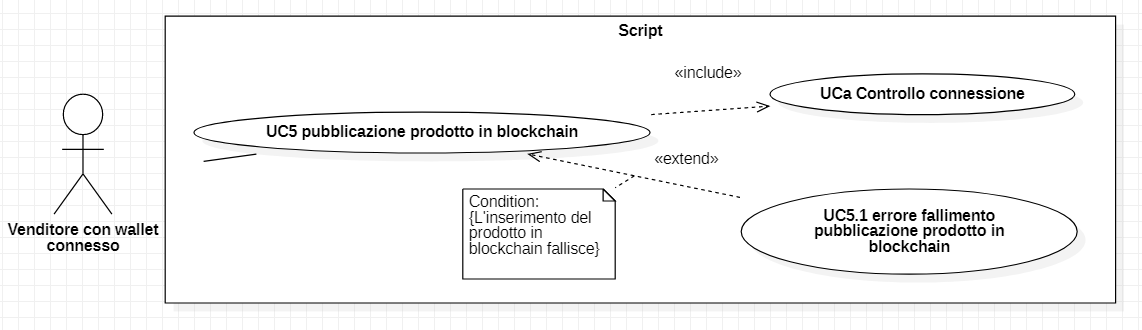
\includegraphics[width=0.9\textwidth]{UC_script}

\paragraph{UC5 - Pubblicazione prodotto in blockchain}\\
\textbf{Attore primario}: Venditore con wallet connesso.\\
\textbf{Precondizioni}: Il venditore ha integrato lo script nell'e-commerce e ha inserito un nuovo prodotto nell'e-commerce.\\
\textbf{Postcondizioni}: Il venditore ha pubblicato il nuovo prodotto in blockchain.\\
\textbf{Scenario principale}:
\begin{enumerate}
    \item il venditore inserisce un nuovo prodotto nell'e-commerce;
    \item tramite lo script il prodotto viene pubblicato in blockchain;
    \item il prodotto è pubblico in blockchain e utilizzabile per fare nuove transazioni.
\end{enumerate}
\textbf{Estensioni}:
\begin{enumerate}
    \item UC5.1 errore fallimento pubblicazione prodotto in blockchain:
    \begin{enumerate}
        \item lo script salva in un file di log il messaggio di errore.
    \end{enumerate}
\end{enumerate}

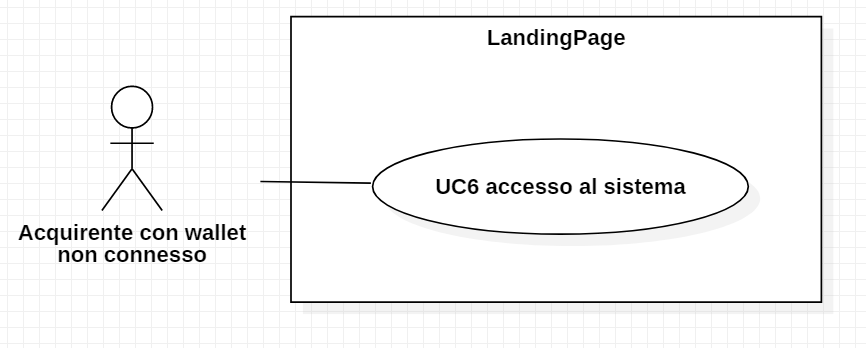
\includegraphics[width=0.9\textwidth]{UC_LP1}

\paragraph{UC6 - Accesso al sistema (landing page)}\\
\textbf{Attore primario}: Acquirente con wallet non connesso.\\
\textbf{Precondizioni}: L'acquirente in landing page non è connesso con metamask.\\
\textbf{Postcondizioni}: L'acquirente accede al sistema.\\
\textbf{Scenario principale}:
L'acquirente usando Metamask, si connette con il proprio wallet.

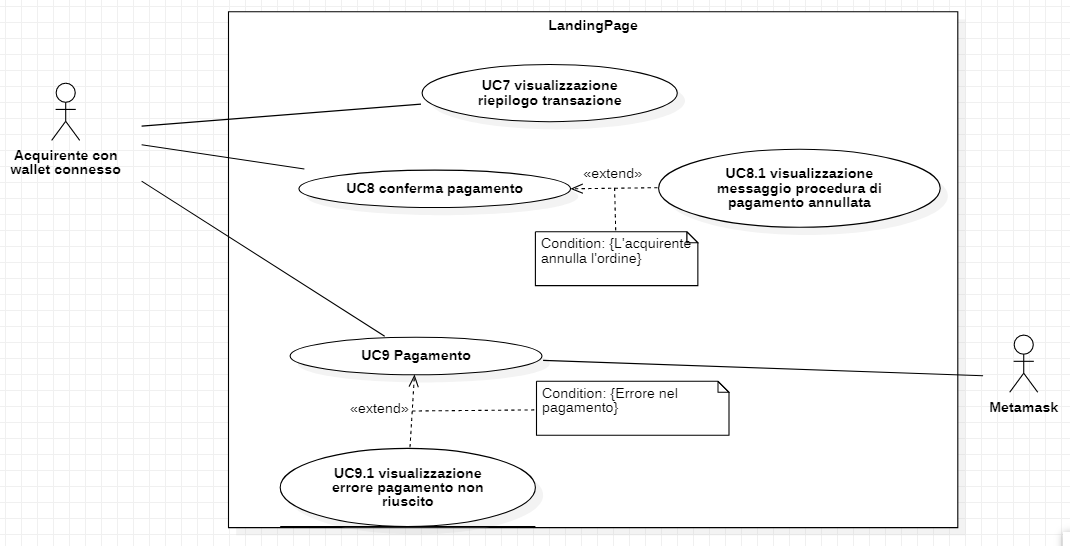
\includegraphics[width=0.9\textwidth]{UC_LP2}

\paragraph{UC7 - Visualizzazione riepilogo transazione}\\
\textbf{Attore primario}: Acquirente con wallet connesso.\\
\textbf{Precondizioni}: L'acquirente con wallet connesso vuole effettuare un acquisto usando ShopChain.\\
\textbf{Postcondizioni}: Il sistema mostra il riepilogo della transazione.\\
\textbf{Scenario principale}:
Viene mostrato all'acquirente il riepilogo della transazione con il prezzo in dollari da pagare.

\paragraph{UC8 - Conferma pagamento}\\
\textbf{Attore primario}: Acquirente riconsocito.\\
\textbf{Precondizioni}: L'acquirente sta effettuando un acquisto e il sistema mostra il riepilogo della transazione.\\
\textbf{Postcondizioni}: L'acquirente ha confermato il pagamento.\\
\textbf{Scenario principale}:
\begin{enumerate}
    \item il sistema mostra il riepilogo della transazione;
    \item l'acquirente conferma l'ordine.
\end{enumerate}
\textbf{Estensioni}:
\begin{enumerate}
    \item UC8.1 Visualizzazione messaggio procedura di pagamento annullata:
    \begin{enumerate}
        \item visualizzazione messaggio procedura di pagamento annullata;
        \item cancellazione sessione di pagamento.
    \end{enumerate}
\end{enumerate}

\paragraph{UC9 - Pagamento}\\
\textbf{Attore primario}: Acquirente con wallet connesso.\\
\textbf{Attore secondario}: Metamask.\\
\textbf{Precondizioni}: L'acquirente ha confermato il pagamento.\\
\textbf{Postcondizioni}: Il pagamento è stato completato con successo.\\
\textbf{Scenario principale}:
\begin{enumerate}
    \item l'acquirente avvia la procedura di pagamento;
    \item l'acquirente effettua il pagamento tramite Metamask;
    \item l'ordine è stato pagato.
\end{enumerate}
\textbf{Estensioni}:
\begin{enumerate}
    \item UC9.1 visualizzazione errore pagamento non riuscito:
    \begin{enumerate}
        \item il pagamento non è stato completato con successo;
        \item cancellazione sessione di pagamento.
    \end{enumerate}
\end{enumerate}

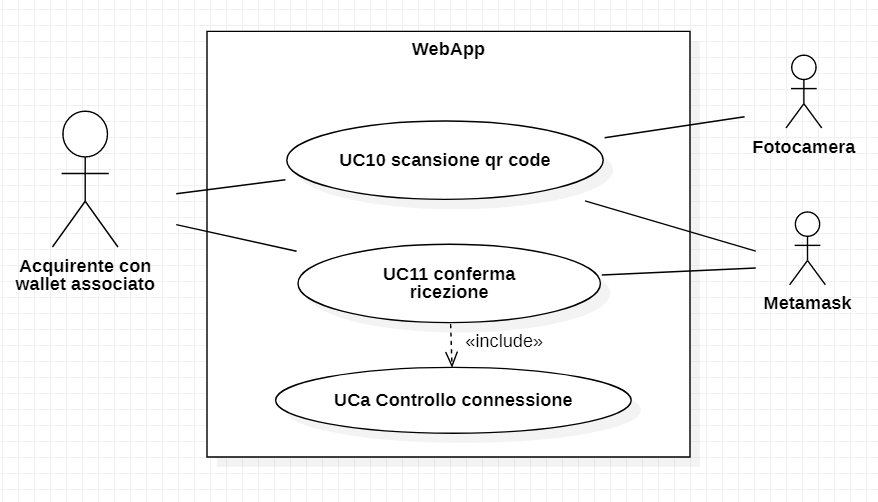
\includegraphics[width=0.9\textwidth]{UC_WAA1}

\paragraph{UC10 - Accesso al sistema (webapp acquirente)}\\
\textbf{Attore primario}: Acquirente con wallet non connesso.\\
\textbf{Precondizioni}: L'acquirente vuole accedere alla webapp.\\
\textbf{Postcondizioni}: L'acquirente si è connesso alla webapp con Metamask.\\
\textbf{Scenario principale}:
L'acquirente usando Metamask si connette alla webapp con il proprio wallet.

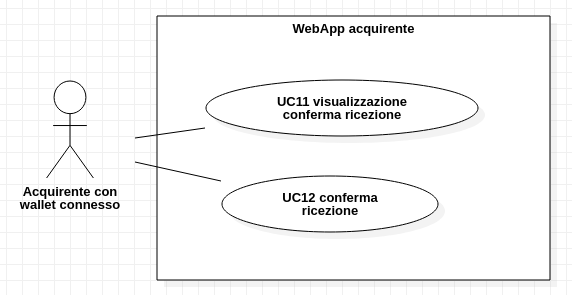
\includegraphics[width=0.9\textwidth]{UC_WAA2}

\paragraph{UC11 - Scansione QR Code}\\
\textbf{Attore primario}: Acquirente con wallet connesso.\\
\textbf{Attori secondari}: Fotocamera, Metamask.\\
\textbf{Precondizioni}: L'acquirente è connesso alla webapp con Metamask.\\
\textbf{Postcondizioni}: L'acquirente ha scansionato il QR Code e viene mandato alla pagina di Metamask della relativa transazione.\\
\textbf{Scenario principale}:
\begin{enumerate}
    \item l'acquirente apre la fotocamera per la scansione del QR Code dalla webapp o da Metamask;
    \item l'acquirente scansiona il QR Code;
    \item viene riconosciuto il link dal QR Code;
    \item viene mostrata la pagina di Metamask della transizione.
\end{enumerate}
\textbf{Estensioni}:
\begin{enumerate}
    \item UC11.1 Visualizzazione errore scansione qr code:
        La fotocamera ha scansionato un QR Code con un link non valido:
        \begin{enumerate}
            \item il sistema mostra l'errore "QR Code non valido";
            \item l'acquirente può ripetere la scansione.
        \end{enumerate}
\end{enumerate}

\paragraph{UC12 - Conferma ricezione}\\
\textbf{Attore primario}: Acquirente riconsciuto.\\
\textbf{Attore secondario}: Metamask.\\
\textbf{Precondizioni}: L'acquirente ha scansionato un QR Code valido.\\
\textbf{Postcondizioni}: L'acquirente ha confermato la ricezione del pacco.\\
\textbf{Scenario principale}:
\begin{enumerate}
    \item l'acquirente scansiona un QR Code valido;
    \item viene mostrata la pagina di Metamask della transizione;
    \item l'acquirente controlla sia tutto corretto e conferma la ricezione del pacco;
    \item il denaro viene sbloccato e mandato nel wallet del venditore.
\end{enumerate}

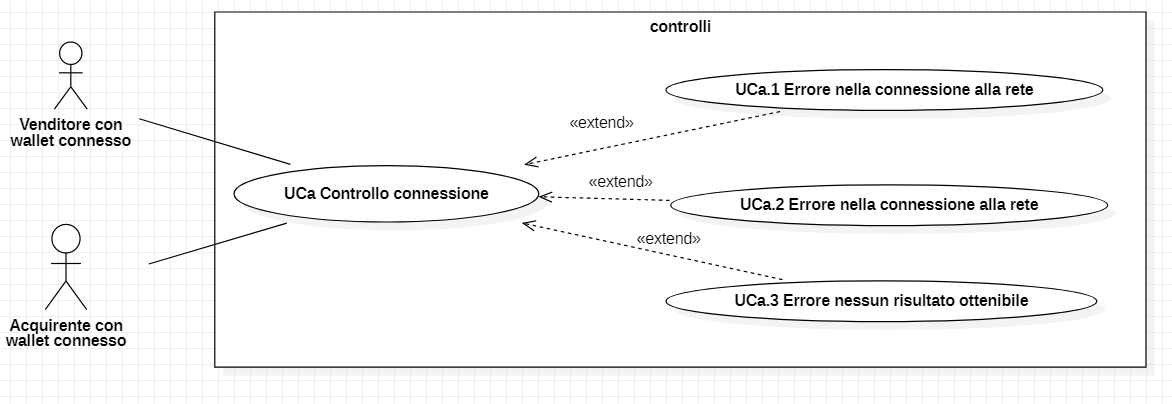
\includegraphics[width=0.9\textwidth]{UC_controlli}

\paragraph{UCa Controllo connessione}\\
\textbf{Attori primari}: Venditore con wallet connesso, Acquirente con wallet connesso. \\
\textbf{Precondizioni}: Il sistema vuole interagire con la blockchain.\\
\textbf{Postcondizioni}:  Il sitema può interagire con la blockchain senza problemi.\\
\textbf{Scenario principale}:
Vengono fatti una serie di controlli per la corretta interazione con la blockchain.\\
\textbf{Estensioni}:
\begin{enumerate}
    \item UCa.1 Errore nella connessione alla rete:\\
        Il venditore o l'acquirente è connesso alla rete sbagliata
    \item UCa.2 Errore transazione non inviata:\\
        La transazione non è stata inviata correttamente.
    \item UCa.3 Errore nessun risultato ottenibile:\\
        La transazione è stata correttamente inviata, ma non è stato ottenuto nessun risultato.
\end{enumerate}

\section{Requisiti}
Ogni requisito è indentificato da un codice univoco composto da: R(per requisito)+F/N(per la tipologia: funzionale, non funzionale)+O/D/F(per la rilevanza: obbligatorio, desiderabile, facoltativo)+x(un numero univoco a due cifre).
\subsection{Requisiti funzionali}
 
 \setlength\tabcolsep{4pt}
\begin{longtable}{|c|p{5cm}|c|c|}
\hline
 \multicolumn{4}{| c |}{Requisiti funzionali}\\
 \hline
 Codice & Descrizione & rilevanza & fonti\\
 \hline
 \endfirsthead

 \hline
 \multicolumn{4}{| c |}{Requisiti funzionali}\\
 \hline
 Codice & Descrizione & Rilevanza & Fonti\\
 \hline
 \endhead

\hline
RFO01 & Il venditore privo di wallet riconosciuto deve poter far riconoscere il proprio wallet tramite Metamask. & Obbligatorio & UC2 \\
\hline
RFO02 & L'acquirente privo di wallet riconosciuto deve poter far riconoscere il proprio wallet tramite Metamask. & Obbligatorio & UC6, UC14 \\
\hline
RFO03 & Il venditore con wallet già associato tramite metamask deve poter accedere automaticamente al sistema. & Obbligatorio & UC7, UC15 \\
\hline
RFO04 & L'acquirente con wallet già associato tramite metamask deve poter accedere automaticamente al sistema. & Obbligatorio & UC7, UC15 \\
\hline
RFO05 & Un utente privo di wallet riconosciuto non può accedere al sistema. & Obbligatorio & Capitolato, decisione interna \\
\hline
RFO06 & Il sistema deve mostrare un messaggio di errore se la procedura di riconoscimento wallet tramite Metamask fallisce. & Obbligatorio & UC3.2, UC11, UC18 \\
\hline
RFO07 & Il venditore deve poter visualizzare la lista delle transazioni. & Obbligatorio & UC3 \\ 
\hline
RFO08 & Il venditore deve poter visualizzare i dettagli di una singola transazione. & Obbligatorio & UC4 \\ 
\hline
RFO09 & Il venditore deve poter visualizzare, per ogni transazione, il suo stato, l'importo, e la scadenza. & Obbligatorio & UC4.1, UC4.3 e UC4.4 \\ 
\hline
RFO10 & Il venditore deve poter generare il QR Code corrispondente ad una certa transazione, direttamente dalla pagina di visualizzazione dei dettagli della stessa. & Obbligatorio & UC4.2 \\ 
\hline
RFO11 & Ad ogni inserimento di un nuovo prodotto nel sito di e-commerce del venditore, in automatico viene inserito lo stesso prodotto in blockchain. & Obbligatorio & UC5 \\ 
\hline
RFO12 & L'acquirente con wallet associato deve poter vedere il riepilogo del'ordine sulla landing page. & Obbligatorio & UC8 \\
\hline
RFO13 & Il costo nel riepilogo ordine sulla landing page deve essere visualizzato in dollari. & Obbligatorio & UC8.1 \\
\hline
RFO14 & L'acquirente con wallet associato deve poter confermare l'ordine sulla landing page. & Obbligatorio & UC9 \\
\hline
RFO15 & Il sistema deve mostrare un messaggio se l'utente annulla l'ordine sulla landing page. & Obbligatorio & UC12 \\
\hline
RFO16 & L'acquirente con wallet associato deve poter pagare l'ordine sulla landing page tramite Metamask. & Obbligatorio & UC10 \\
\hline
RFO17 & Il sistema deve mostrare un messaggio di errore se la procedura di pagamento sulla landing page tramite Metamask fallisce. & Obbligatorio & UC13 \\
\hline
RFO18 & L'acquirente con wallet associato deve poter scansionare il QR Code sulla webapp. & Obbligatorio & UC16 \\
\hline
RFO19 & Il sistema deve mostrare un messaggio di errore se la procedura di scansione QR Code nella webapp fallisce. & Obbligatorio & UC19 \\
\hline
RFO20 & L'acquirente con wallet associato deve poter accettare l'ordine sulla webapp tramite Metamask. & Obbligatorio & UC17 \\
\hline
RFO21 & Il sistema deve mostrare un messaggio di errore se la procedura di accettazione ordine nella webapp tramite Metamask fallisce. & Obbligatorio & UC20 \\
\hline

\end{longtable}
\pagebreak

\setlength\tabcolsep{4pt}
\begin{longtable}{|c|p{5cm}|c|c|}
\hline
 \multicolumn{4}{| c |}{Requisiti non funzionali}\\
 \hline
 Codice & Descrizione & rilevanza & fonti\\
 \hline
 \endfirsthead

 \hline
 \multicolumn{4}{| c |}{Requisiti non funzionali}\\
 \hline
 Codice & Descrizione & Rilevanza & Fonti\\
 \hline
 \endhead

\hline
RNO22 & Utilizzo di blockchain pubblica. & Obbligatorio & Capitolato, decisione interna \\
\hline
RND23 & Utilizzo di Java e Angular per lo sviluppo delle parti di Back-end e di Front-end
della componente web application del sistema. & Desiderabile &  Capitolato\\
\hline
RND24 & Utilizzo di database PostgreSQL. & Desiderabile & Capitolato \\
\hline
RND25 & Utilizzo di Java e Angular per lo sviluppo delle parti di Back-end e di Front-end
della componente web application del sistema. & Desiderabile &  Capitolato\\
\hline
RNO26 & Il venditore deve disporre di un manuale utente per l'utilizzo del sistema. & Obbligatorio &  UC1, decisione interna\\
\hline
RNO27 & Test che dimostrino il corretto funzionamento dei servizi e delle funzionalità previste,
con una copertura minima dell’ 80\% correlata di report. & Obbligatorio & Capitolato\\
\hline
RNO28 & Documentazione su scelte implementative e progettuali effettuate, le relative motivazioni, i problemi aperti e le eventuali soluzioni proposte da esplorare. & Obbligatorio & Capitolato\\
\hline
RNO29 & Deve essere reso disponibile uno script python scaricabile dai venditori da integrare nel loro e-commerce per l'invio automatico dei nuovi prodotti in BlockChain. & Obbligatorio & UC5, decisione interna\\
\hline

\end{longtable}



\end{document}